\section{Definitions}
\label{Sect:SciFiDefinitions}

\subsection{Labelling of upstream and downstream trackers}
\label{SubSect:SciFiTkrLabel}

The official labels for the two trackers are: 
\begin{eqnarray}
  {\rm Upstream~tracker}   & \rightarrow & {\rm Tracker \# 1} \nonumber \\
  {\rm Downstream~tracker} & \rightarrow & {\rm Tracker \# 2} \nonumber 
\end{eqnarray}
The internals of the code however will frequently refer to the upstream tracker as 0, and the downstream tracker as 1. In this document, we will use the official convention.

\subsection{Station numbering}
\label{SubSect:SciFiStnNumbering}

The tracker reference document defines the station ``labelling'' of the stations in relation to the focus-coil module that is immediately downstream of tracker 1 or, equivalently, immediately upstream of tracker 2.  The station closest to the focus-coil module in question is labelled  ``1''.  The label then increases such that station 5 is the station
closest to the optical patch panel. The scheme is summarised in table~\ref{Tab:StnNum} and figure~\ref{Fig:StnNum}.

\begin{table}[hb]
  \caption{Station numbering scheme. The ``label'' of the stations that make up a MICE tracker runs from 1 to 5. The location of the station in relation to the patch panel and the absorber is reported in the column labelled ``Location''.}
  \label{Tab:StnNum}
  \begin{tabular}{|l|r|}
    \hline
    {\bf Location}                                  & {\bf Label} \\
    \hline
    Closest to absorber (furthest from patch panel) &           1 \\
                                                    &           2 \\ 
                                                    &           3 \\
                                                    &           4 \\
    Furthest from absorber (closest to patch panel) &           5 \\
    \hline
  \end{tabular}
\end{table}

\begin{figure}
  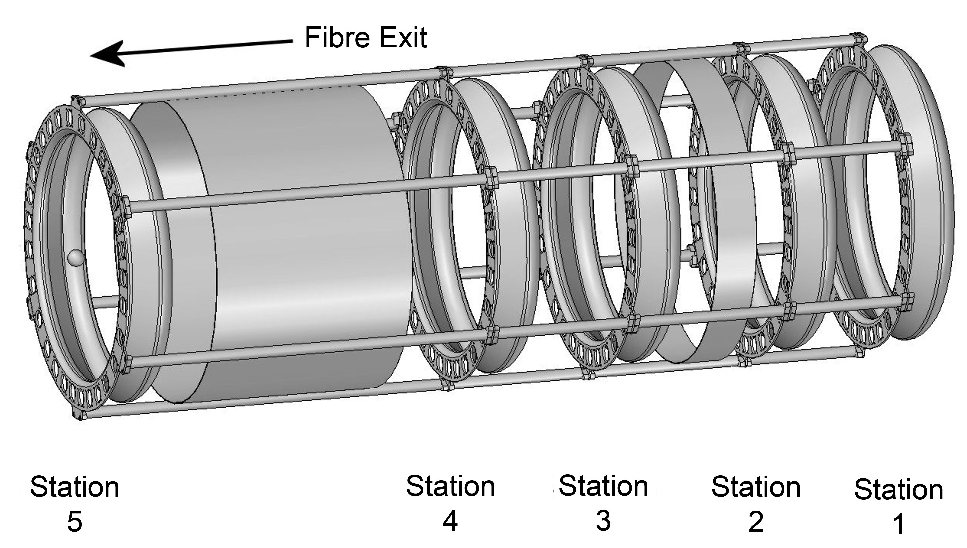
\includegraphics[width=0.6\textwidth]{detectors/tracker/02-Definitions/Figures/StnNum.pdf}
  \caption{Schematic diagram of the MICE tracker. The five stations are shown supported by the carbon-fibre space frame, with fibres omitted for clarity. The station numbering scheme is indicated together with the direction in which the clear-fibre light-guides leave the tracking volume.}
  \label{Fig:StnNum}
\end{figure}

\subsection{Doublet layer}
\label{SubSect:SciFiDblLyr}

Each station consists of three ``doublet layers'' of 350\,$\mu$m scintillating fibres glued onto a carbon-fibre station body. The doublet layers are labelled $u$ (sometimes refered to also as $x$), $w$ and $v$.  The layers are arranged such that the fibres in one layer run at an angle of 120$^\circ$ to the fibres in each of the other layers as shown in figure \ref{Fig:DblLyr}a.   The arrangement of the fibres within a doublet layer is shown in figure \ref{Fig:DblLyr}b.   The configuration of the seven fibres ganged for readout via a single clear-fibre light-guide is also indicated. % The construction of the doublet layer is described in \cite{TrackerPaper} along with the specification of the various materials of which it is composed.
\begin{figure}
  \begin{center}
    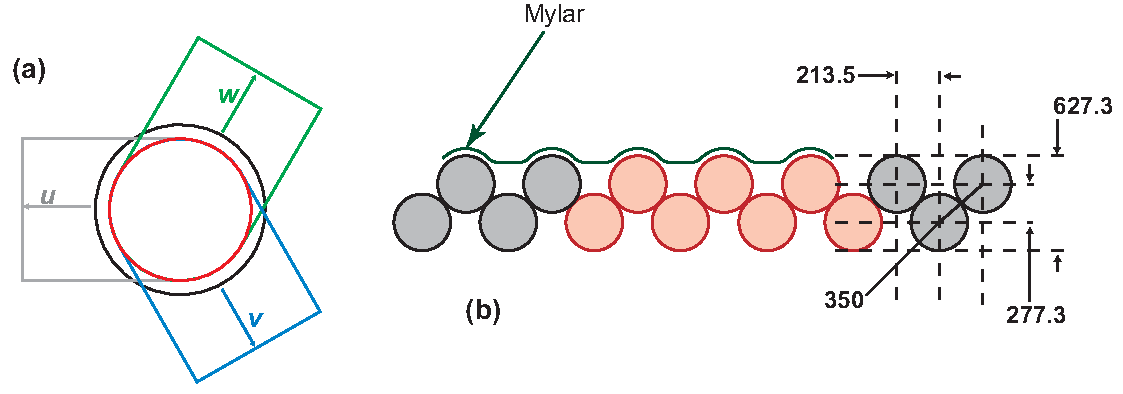
\includegraphics[width=0.7\textwidth]{detectors/tracker/02-Definitions/Figures/doublet-layer.pdf}
  \end{center}
  \caption{(a) Arrangement of the doublet layers in the scintillating-fibre  stations. The outer circle shows the solenoid bore while the inner circle shows the limit of the active area of the tracker. The grey, blue, and green regions indicate the direction that the individual 350\,$\mu$m fibres run (moving outward from the centre) in the $u$, $v$, and $w$ planes respectively. (b) Detail of the arrangement of the scintillating fibres in a doublet layer. The fibre spacing and the fibre pitch are indicated on the right-hand end of the figure in \,$\mu$m. The pattern of seven fibres ganged for readout in a single clear-fibre light-guide is shown in red. The sheet of Mylar glued to the doublet layer is indicated.}
  \label{Fig:DblLyr}
\end{figure}

\subsubsection{Doublet-layer numbering}
\label{SubSubSect:SciFiDblNmbrng}

The order in which the doublet layers were glued onto the station body is shown in figure~\ref{Fig:DblLyrOrder}. The $u$ layer was glued to the station body first. The doublet layer was glued such that the ``fibre side'' of the doublet layer was glued to the station body; i.e. the mylar sheet faces away from the station body. The $w$ layer was then glued onto the outer surface of the $u$ layer. The fibre side of the $w$ layer was glued to the mylar sheet of the $u$ layer such that the mylar sheet of the $w$ layer also faces away from the station body. Finally, the $v$ layer was glued onto the assembly. The gluing arrangement was the same as for the $u$ and $w$ layers, i.e. the mylar sheet of the $v$ layer also faces away from the station body. 

%The numbering of the layers, which follows the order in which the layers were glued onto the station body, is summarised in table \ref{Tab:DblLyrOrder}.

\begin{figure}
  \begin{center}
    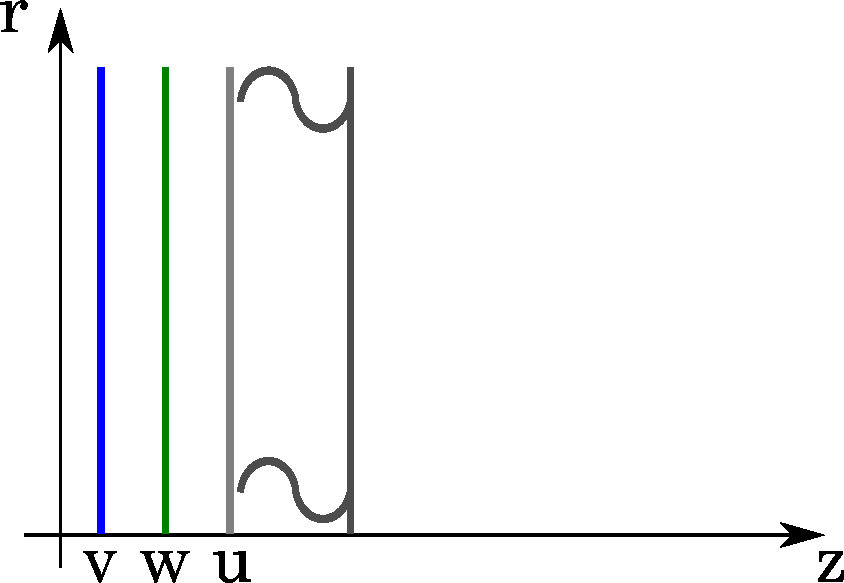
\includegraphics[width=0.65\linewidth]{detectors/tracker/02-Definitions/Figures/doublet-layer-order.pdf}
  \end{center}
  \caption{ The order in which the doublet layers were glued onto the station body.The station body is indicated by the solid black lines. The $u$ layer (shown as the grey line was glued to the station body first. The $w$ (indicated by the green line) was then glued onto the outer surface of the $u$ layer.  The outer doublet layer, the $v$ layer (shown as the blue line) was then glued onto the assembly. The station reference surface and the direction of increasing $z$  are shown as the thin black lines.}
  \label{Fig:DblLyrOrder}
\end{figure}

% \begin{table}
%   \caption{Doublet-layer numbering scheme.  The doublet-layer ``number'' runs from 0 to 2. The correspondence between the doublet layer number and the  view is reported in the column labelled ``Doublet-layer number''.}
%   \label{Tab:DblLyrOrder}
%   \begin{tabular}{|l|r|}
%     \hline
%     {\bf View} & {\bf Double-layer number} \\
%     \hline
%     $u$        &                         0 \\
%     $w$        &                         1 \\
%     $v$        &                         2 \\
%     \hline
%   \end{tabular}
% \end{table}

\subsection{Fibre-channel numbering}
\label{SubSect:SciFiFbrNmbrng}

The numbering of the groups of seven fibres ganged for readout is shown in figure \ref{Fig:FbrChnlNmbrng}. With the mylar surface facing up, and with the tails leading out to the station connectors taken to be at the bottom of the figure, the fibre-channel increases from left to right. The coordinate measured by the doublet layer ($u$, $v$ or $w$) is taken to increase in the same direction as the channel number. The origin of the measured coordinate is taken to be at the position of the central fibre.

\begin{figure}
  \begin{center}
    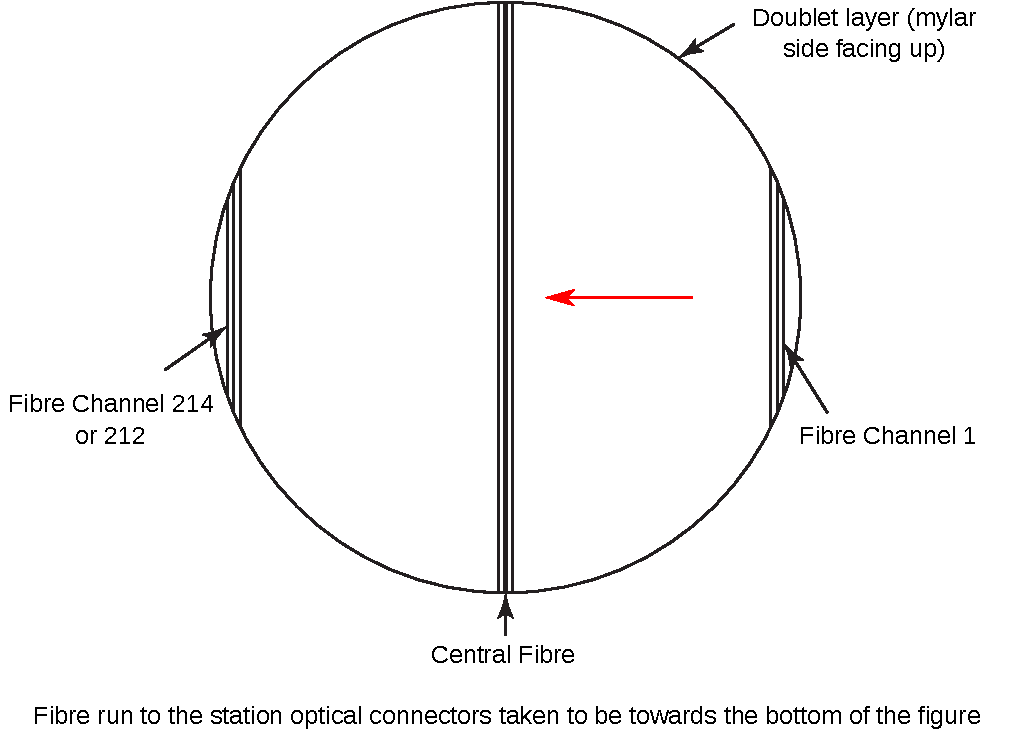
\includegraphics[width=0.85\linewidth]{detectors/tracker/02-Definitions/Figures/fibre-channel-numbering.pdf}
  \end{center}
  \caption{The order in which fibre channels (groups of seven fibres) are numbered. The sensitive surface of the doublet layer is indicated by the solid circle. The direction in which the fibres run is indicated by the vertical lines. The station optical connectors are taken to be at the bottom of the figure as indicated. With the mylar sheet taken to be facing up, fibre-channel number 1 is to the left of the central fibre. The fibre-channel number increases from left to right. The ``zero'' of the coordinate ($u$, $v$ or $w$ increases) measured by the doublet layer is taken to be the position of the central fibre. The direction in which the coordinate measured by the double layer increases is indicated by the red arrow.}
  \label{Fig:FbrChnlNmbrng}
\end{figure}
